%%%%%%%%%%%%%%%%%%%%%%%%%%%%%%%%%%%%%%%%%%%%%%%%%%%%%%%%
%%%%%%%%%%%%%%%%%%%%%%%%%%%%%%%%%%%%%%%%%%%%%%%%%%%%%%%%
%%%                                                  %%%
%%% University of Arizona themed Beamer presentation %%%
%%% Based on the Warsaw, Palo Alto and UNL templates %%%
%%% modified by Joseph V. Casillas (6-13-2011)       %%%
%%%                                                  %%%
%%%%%%%%%%%%%%%%%%%%%%%%%%%%%%%%%%%%%%%%%%%%%%%%%%%%%%%%
%%%%%%%%%%%%%%%%%%%%%%%%%%%%%%%%%%%%%%%%%%%%%%%%%%%%%%%%

\documentclass{beamer}
\mode<presentation>{\usetheme{UA3}\setbeamercovered{transparent}}
\usepackage{ling}
\usepackage{verbatim}
\usepackage{media9}
\usepackage{tikz}
\usepackage{tikz-qtree}

\title{Percepción del habla}

\author[Casillas]{Joseph Casillas}

\institute{Universidad de Arizona}

\date{Semana 9}

\subject{Linguistics}

\begin{document}

%%%%%%%%%%%%%%%%%%%%%%%%%%%%%%%%%
%%%%%%%%%%%%%%%%%%%%%%%%%%%%%%%%%
\begin{frame}%Página principal
  \titlepage
\end{frame}


\begin{frame}
\frametitle{La percepción del habla}

	\begin{itemize}
		\item El proceso de recibir e interpretar el habla
		\item El inverso de la producción
	\end{itemize}
\end{frame}

\begin{frame}[plain]

	\begin{center}
		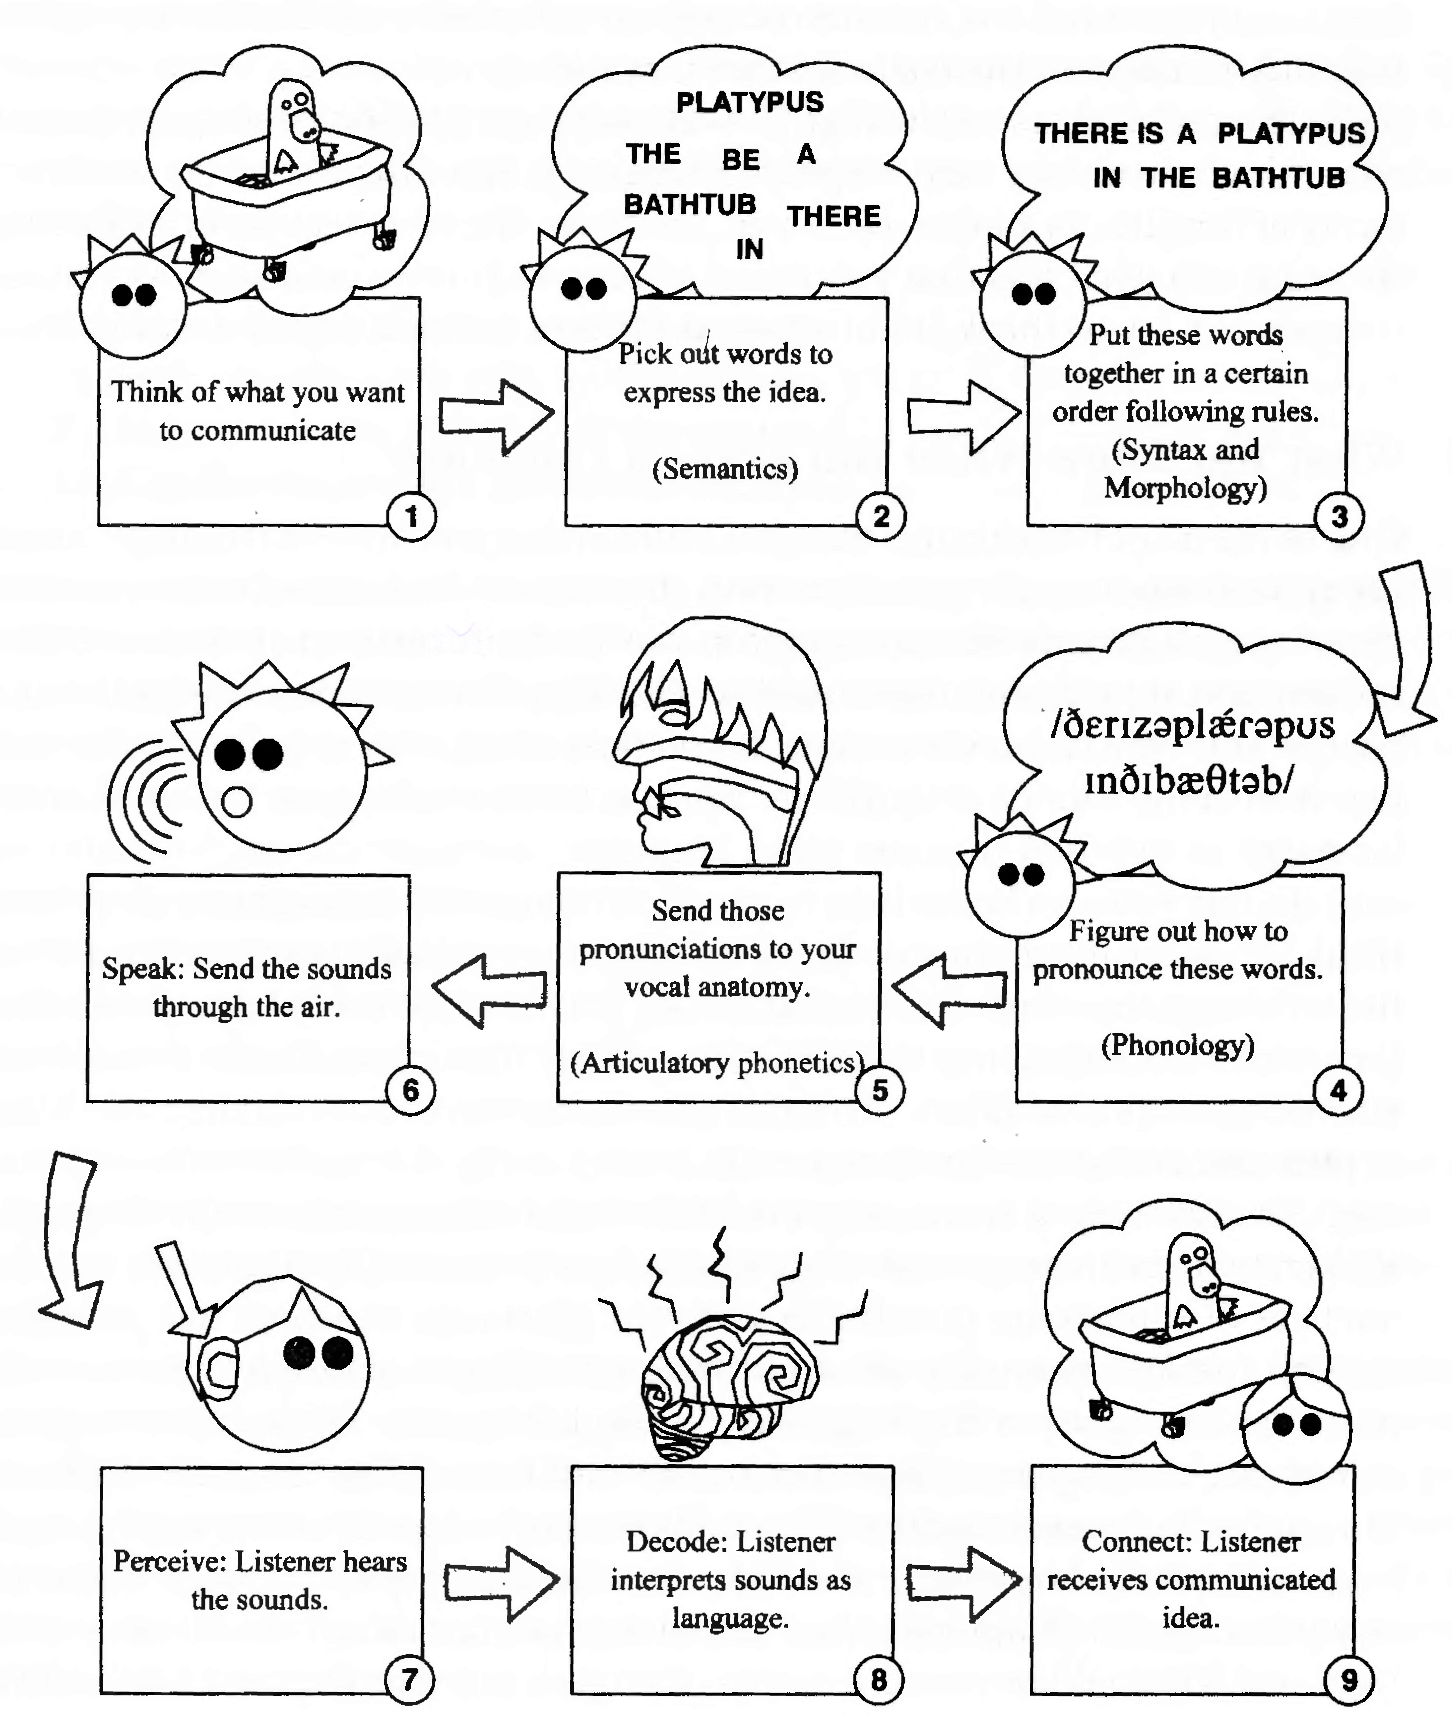
\includegraphics[width=.6\textwidth]{figures/cadena_hablada.png}
	\end{center}
\end{frame}

\begin{frame}
	\frametitle{La percepción del habla}
	
	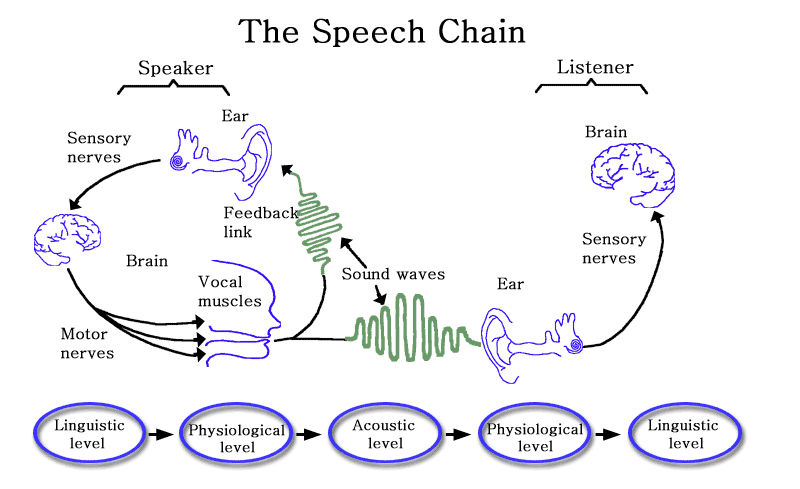
\includegraphics[width=\textwidth]{figures/cadena_hablada2.png}
\end{frame}

\begin{frame}
	\frametitle{La percepción del habla}

	\begin{itemize}
		\item ¿Cómo decodificamos la señal acústica?
		\item Percibimos e interpretamos los sonidos del habla muy rápidamente (en milisegundos)
		\item Asociamos los sonidos con las palabras que tenemos en nuestro lexicón
		\item Aplicamos las reglas sintácticas de nuestra lengua para entender el mensaje
	\end{itemize}
\end{frame}

\begin{frame}
	\frametitle{La percepción del habla}
	
	\begin{itemize}
		\item ¿Cómo diferenciamos entre el habla y el ruido?
		\item ¿Cómo extraemos la información relevante de una señal pobre?
		\item Los sonidos del habla nunca se pronuncian de la misma forma
	\end{itemize}
\end{frame}

\begin{frame}
	\frametitle{La percepción del habla}
	\framesubtitle{La ausencia de invarianza}

	\begin{itemize}
		\item Los sonidos del habla nunca se pronuncian de la misma forma
		\item Si digo ``taco'' \textipa{[\textprimstress ta.ko]} 10 veces, nunca es físicamente igual 
		\item ¿Cómo es que somos capaces de relacionar el sonido con el concepto de un fonema?
	\end{itemize}

\end{frame}

\begin{frame}
	\frametitle{La percepción del habla}
	\framesubtitle{La percepción categórica}

	\begin{itemize}
		\item ``Equal sized physical differences are not equal sized psychologically.''
		\item No percibimos los continuos como continuos\ldots
		\item Las diferencias dentro de la misma categoría se disminuyen 
		\item Las diferencias entre categorías se aumentan
	\end{itemize}
\end{frame}

\begin{frame}
	\frametitle{La percepción del habla}
	\framesubtitle{La percepción categórica}

	\begin{center}
		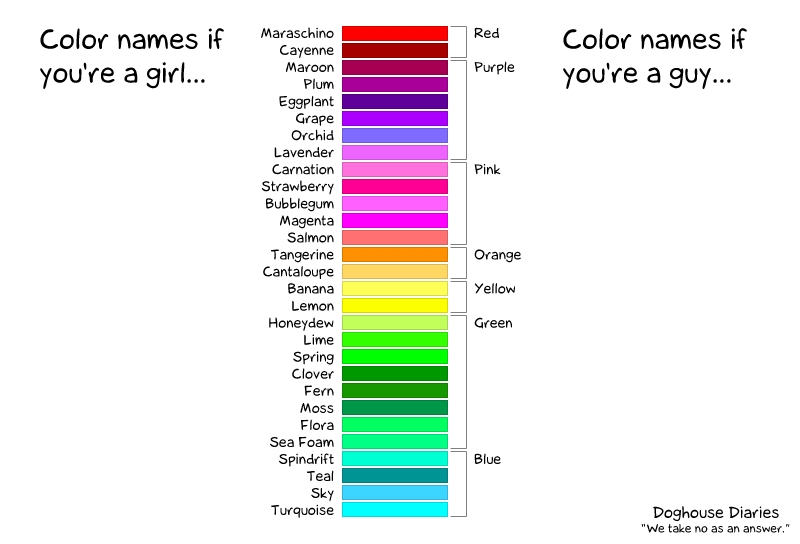
\includegraphics[width=.8\textwidth]{figures/colors.png}
	\end{center}
\end{frame}

\begin{frame}
	\frametitle{La percepción del habla}
	\framesubtitle{La percepción categórica}

	\begin{center}
		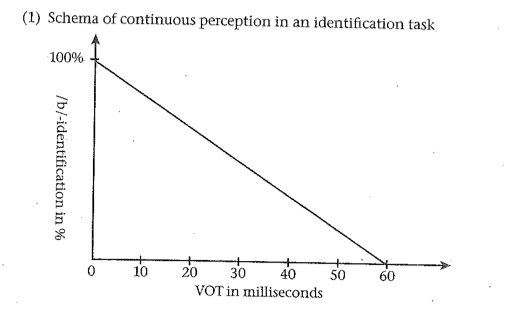
\includegraphics[scale=.3]{figures/pc1.png} 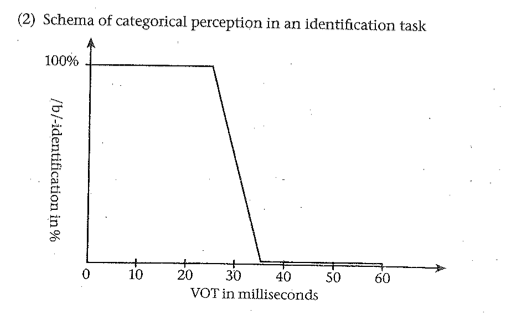
\includegraphics[scale=.3]{figures/pc2.png}
	\end{center}
\end{frame}

\begin{frame}[plain]
	\begin{center}
		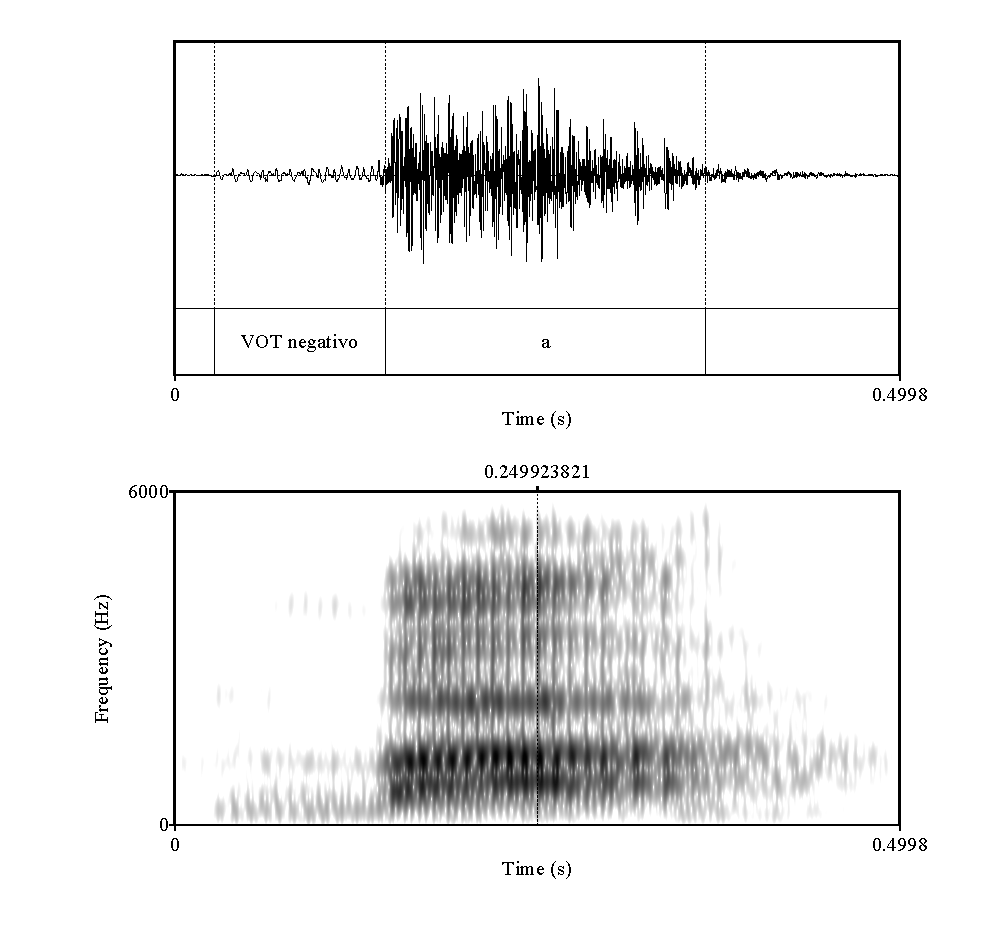
\includegraphics[scale=.28]{figures/baNEG.pdf} 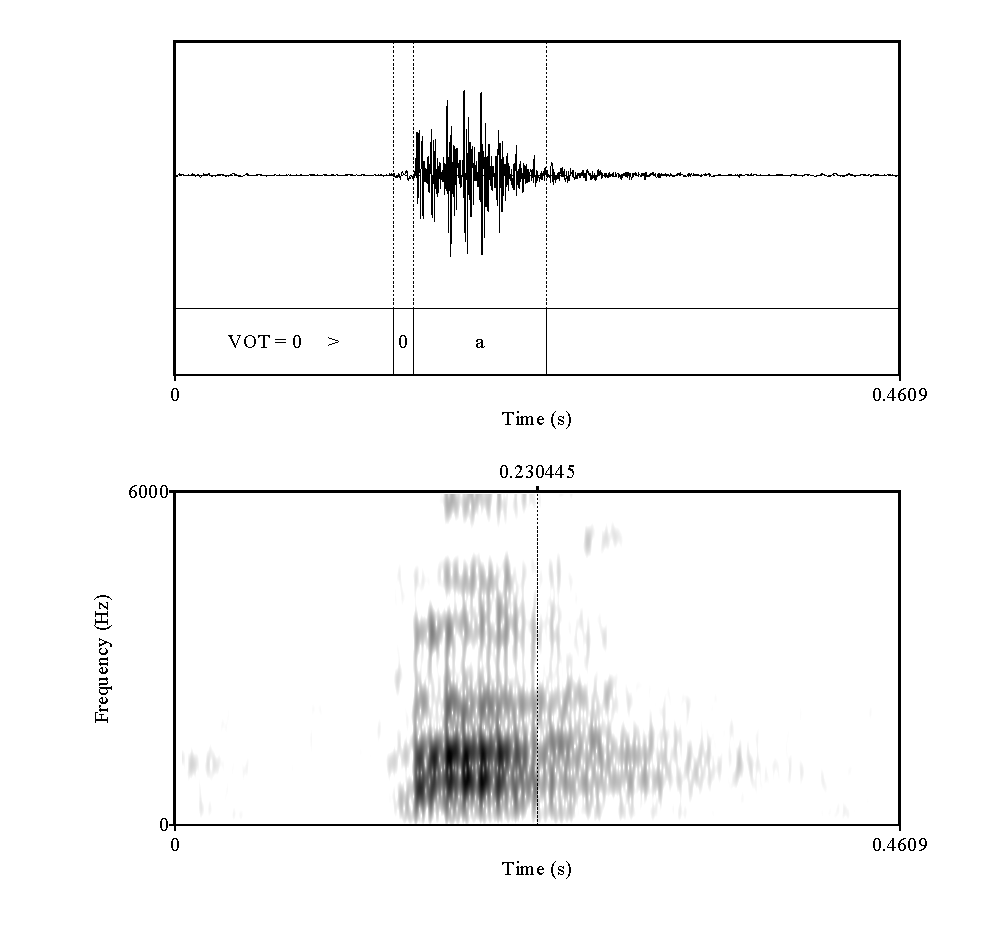
\includegraphics[scale=.28]{figures/pa0.pdf} 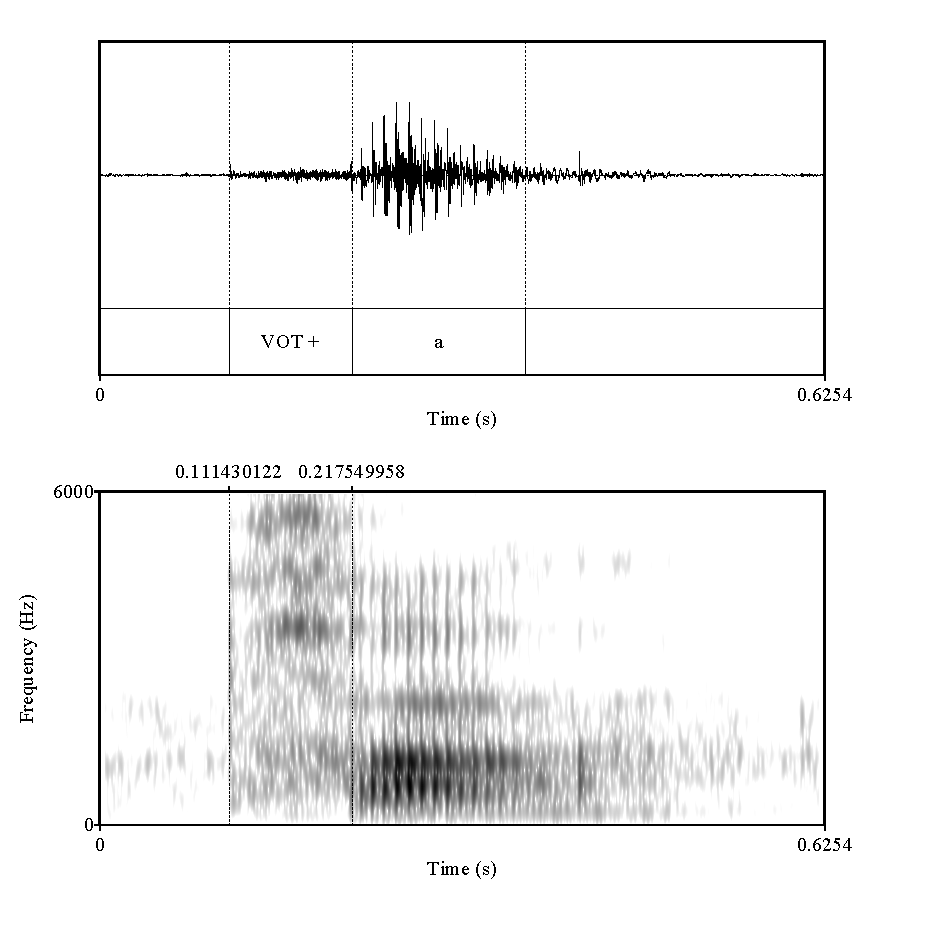
\includegraphics[scale=.28]{figures/paPOS.pdf}
	\end{center}
\end{frame}

\begin{frame} 
	\frametitle{La percepción del habla}
	\framesubtitle{Con un compañero}
	
	\begin{enumerate}
		\item ¿Qué es VOT? ¿Cómo difiere /b/ de /p/? ¿Y /t/ (español) de /t/ (inglés)? 
		\item ¿Qué significa ``la ausencia de invarianza''? ¿Por qué supone un problema a la hora de explicar la percepción del habla?
		\item En vuestras propias palabras, ¿qué es la percepción categórica?
		\item Explícale a tu vecino cómo funciona un experimento 2AFC (2-alternative forced choice).
	\end{enumerate}
\end{frame}

\begin{frame}[plain]
	\begin{center}
		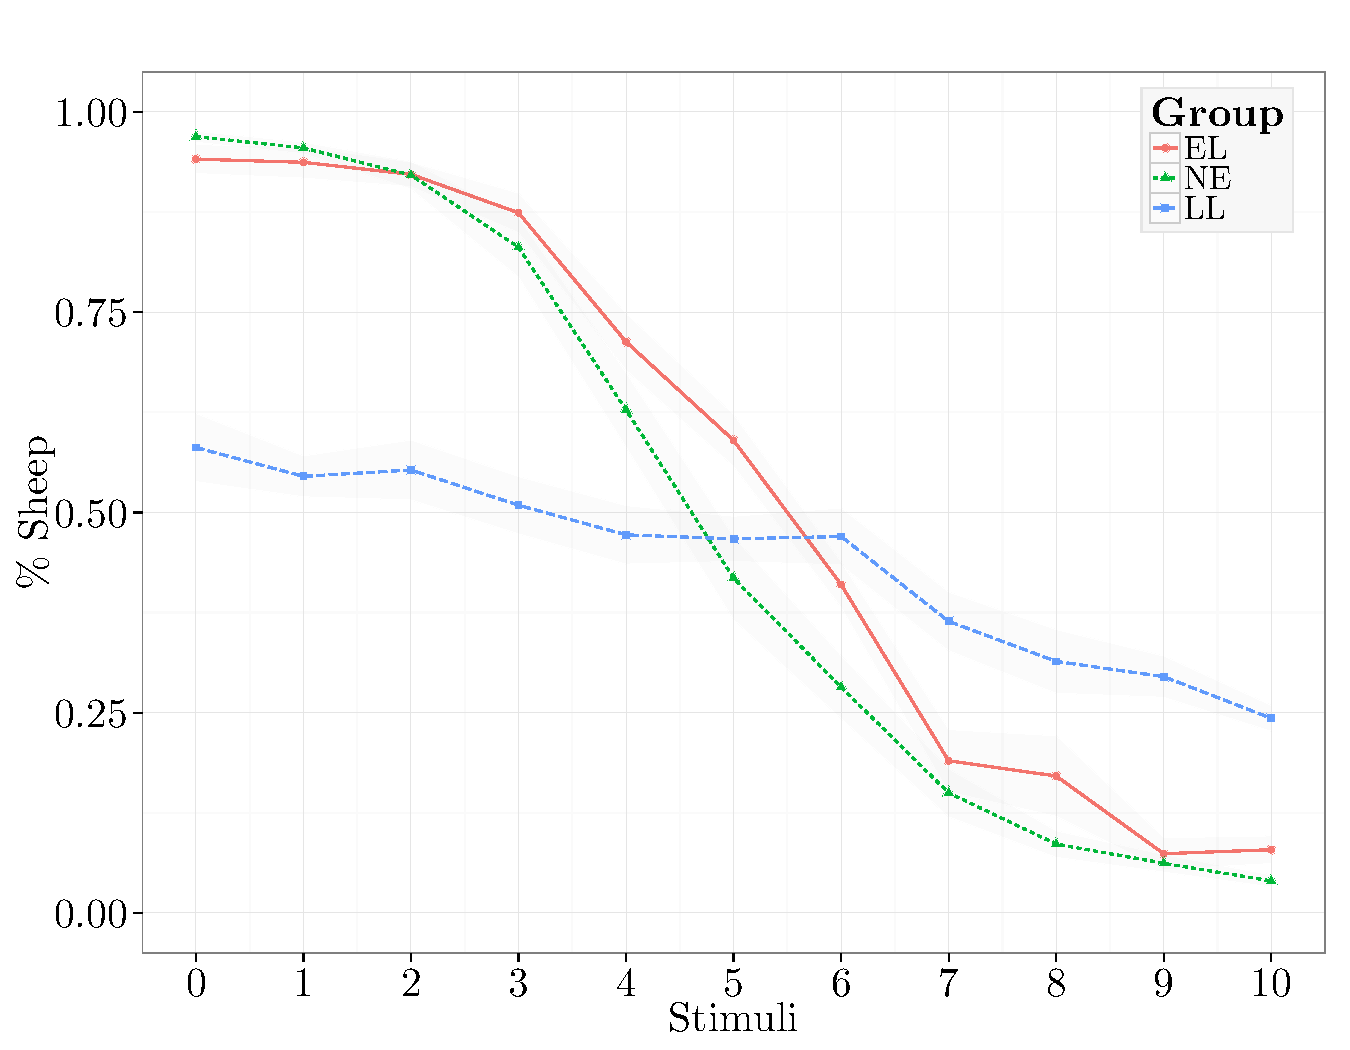
\includegraphics[width=\textwidth]{figures/spec_pro.pdf}
	\end{center}
\end{frame}

\begin{frame} 
	\frametitle{La percepción del habla}
	\framesubtitle{La discriminación}
	
	\begin{center}
		\begin{tabular}{ccc}
		/b/ & 0 -- 1  -- 2  --  3 -- 4  --  5 -- 6  --  7 -- 8  --  9 -- 10 & /p/ \\
		\end{tabular}
	\end{center}
\end{frame}

\begin{frame} 
	\frametitle{La percepción del habla}
	\framesubtitle{La discriminación}
	
	\begin{center}
		\begin{tabular}{ccc}
		/b/ & \textbf{0} -- 1 -- \textbf{2} -- 3 -- 4  --  5 -- 6  --  7 -- 8  --  9 -- 10 & /p/ \\
		\end{tabular}
	\end{center}
\end{frame}

\begin{frame} 
	\frametitle{La percepción del habla}
	\framesubtitle{La discriminación}
	
	\begin{center}
		\begin{tabular}{ccc}
		/b/ & 0 -- \textbf{1} -- 2  -- \textbf{3} -- 4 --  5 -- 6  --  7 -- 8  --  9 -- 10 & /p/ \\
		\end{tabular}
	\end{center}
\end{frame}

\begin{frame} 
	\frametitle{La percepción del habla}
	\framesubtitle{La discriminación}
	
	\begin{center}
		\begin{tabular}{ccc}
		/b/ & 0 -- 1 -- \textbf{2} -- 3 -- \textbf{4}  -- 5 -- 6  --  7 -- 8  --  9 -- 10 & /p/ \\
		\end{tabular}
	\end{center}
\end{frame}

\begin{frame} 
	\frametitle{La percepción del habla}
	\framesubtitle{La discriminación}
	
	\begin{center}
		\begin{tabular}{ccc}
		/b/ & 0 -- 1  -- 2  --  \textbf{3} -- 4 -- \textbf{5} -- 6 --  7 -- 8  --  9 -- 10 & /p/ \\
		\end{tabular}
	\end{center}
\end{frame}

\begin{frame}[t]
	\frametitle{La percepción del habla}
	\framesubtitle{La discriminación}
	
	\begin{center}
		\begin{tabular}{ccc}
		/b/ & 0 -- 1  -- 2  --  3 -- 4  --  5 -- 6  --  7 -- 8  --  9 -- 10 & /p/ \\
		\end{tabular}
	\end{center}

	\begin{center}
		\begin{tabular}{l}
		0 - 2 \\
		1 - 3 \\ 
		2 - 4 \\ 
		3 - 5 \\ 
		4 - 6 \\ 
		5 - 7 \\ 
		6 - 8  \\
		7 - 9  \\
		8 - 10 \\
		\end{tabular}
	\end{center}
\end{frame}

\begin{frame}[t]
	\frametitle{La percepción del habla}
	\framesubtitle{La discriminación}
	
	\begin{center}
		\begin{tabular}{ccc}
		/b/ & 0 -- 1  -- 2  --  3 -- \textbf{4}  --  \textbf{5} -- \textbf{6}  -- 7 -- 8 --  9 -- 10 & /p/ \\
		\end{tabular}
	\end{center}

	\begin{center}
		\begin{tabular}{l}
		0 - 2 \\
		1 - 3 \\ 
		2 - 4 \\ 
		\textbf{3 - 5} \\ 
		\textbf{4 - 6} \\ 
		\textbf{5 - 7} \\ 
		6 - 8  \\
		7 - 9  \\
		8 - 10 \\
		\end{tabular}
	\end{center}
\end{frame}

\begin{frame}[plain]
	\begin{center}
		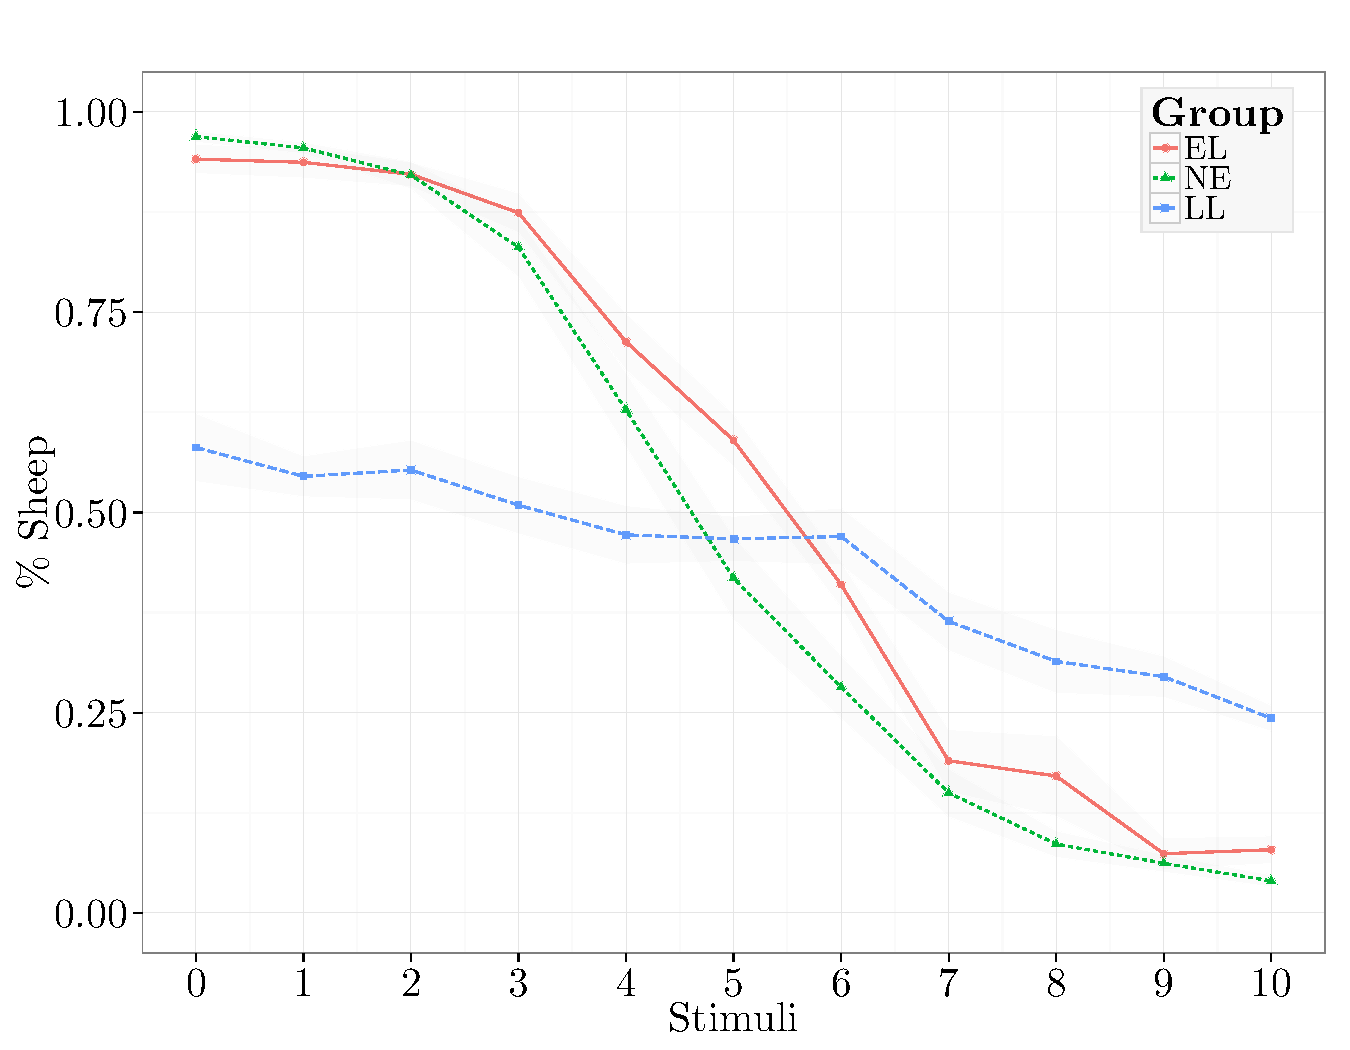
\includegraphics[width=\textwidth]{figures/spec_pro.pdf}
	\end{center}
\end{frame}

\begin{frame}[plain]
	\begin{center}
		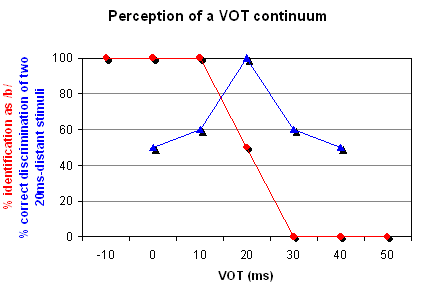
\includegraphics[width=\textwidth]{figures/pc3.png}
	\end{center}
\end{frame}

\begin{frame}
	\frametitle{La percepción del habla}
	\framesubtitle{La percepción categórica}

	\begin{itemize}
		\item ``Equal sized physical differences are not equal sized psychologically.''
		\item No percibimos los continuos como continuos\ldots
		\item Las diferencias dentro de la misma categoría se disminuyen 
		\item Las diferencias entre categorías se aumentan
	\end{itemize}
\end{frame}

\begin{frame} 
	\frametitle{La percepción del habla}
	\framesubtitle{El reconocimiento de las palabras}
	
	\begin{itemize}
		\item Reconocemos las palabras sin esfuerzo 
		\begin{itemize}
			\item El significado semántico
			\item La categoría sintáctica
			\item El significado pragmático
		\end{itemize}
		\item Un niño de 6 años ya sabe 14,000 palabras
		\item Un adulto que ha terminado la universidad sabe 60,000 palabras
	\end{itemize}
\end{frame}

\begin{frame} 
	\frametitle{La percepción del habla}
	\framesubtitle{Frequencia, recencia y conexto}
	
	\begin{itemize}
		\item Viene del trabajo de Ebbinghaus \footnote{El efecto de la posición serial}
		\item Reconocemos más rápidamente las palabras que\ldots 
		\begin{itemize}
			\item ocurren con más frequencia
			\item hemos escuchado recientemente 
			\item vienen después de otras palabras que establecen el contexto
		\end{itemize}
	\end{itemize}
\end{frame}

\begin{frame} 
	\frametitle{La percepción del habla}
	\framesubtitle{Frequencia, recencia y conexto}
	
	\begin{center}
		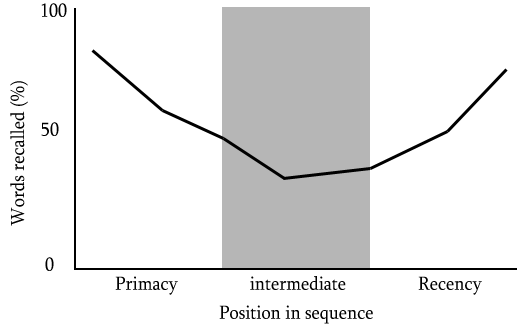
\includegraphics[width=.7\textwidth]{figures/serial_position.png}
	\end{center}
\end{frame}

\begin{frame} 
	\frametitle{La percepción del habla}
	\framesubtitle{Acceso léxico}
	
	\begin{itemize}
		\item ``La palabra es \_\_\_\_\_\_\_''
	\end{itemize}
\end{frame}

\begin{frame} 
	\frametitle{La percepción del habla}
	\framesubtitle{Tareas offline/online}
	
	\begin{itemize}
		\item Offline: se mide el resultado de la tarea
		\begin{itemize}
			\item 2AFC (\% correcto)
			\item Discriminación (\% correcto)
			\item Acceso léxico (\% correcto)
		\end{itemize} 
		\vspace{.2in}
		\item Online: se mide el proceso
		\begin{itemize}
			\item tiempo de reacción
			\item fMRI
			\item ERP
			\item eye-tracking
		\end{itemize}
	\end{itemize}
\end{frame}


\end{document}